\documentclass[10pt]{article}
\usepackage[polish]{babel}
\usepackage[utf8]{inputenc}
\usepackage[T1]{fontenc}
\usepackage{graphicx}
\usepackage[export]{adjustbox}
\graphicspath{ {./images/} }
\usepackage{amsmath}
\usepackage{amsfonts}
\usepackage{amssymb}
\usepackage[version=4]{mhchem}
\usepackage{stmaryrd}

\newcommand\Varangle{\mathop{{<\!\!\!\!\!\text{\small)}}\:}\nolimits}

\begin{document}

\includegraphics[max width=\textwidth, center]{2024_11_21_6a8be49478f78d0689cfg-01(1)}\\
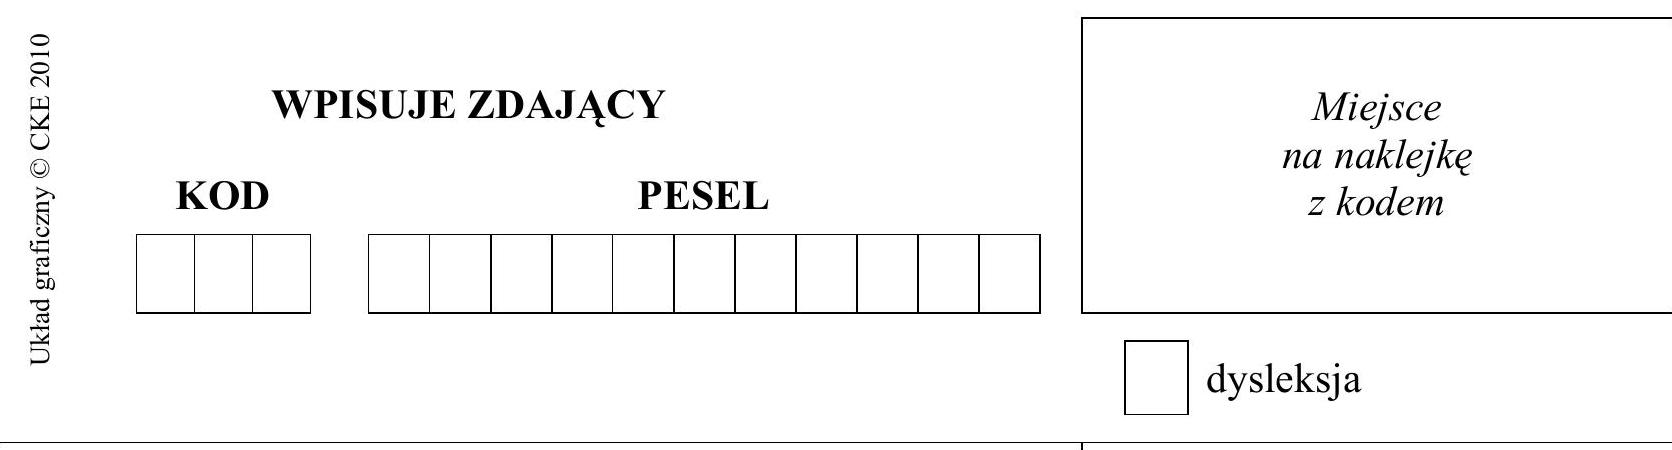
\includegraphics[max width=\textwidth, center]{2024_11_21_6a8be49478f78d0689cfg-01(2)}

\section*{EGZAMIN MATURALNY \\
 Z MATEMATYKI \\
 POZIOM PODSTAWOWY}
\begin{enumerate}
  \item Sprawdź, czy arkusz egzaminacyjny zawiera 20 stron (zadania 1-34). Ewentualny brak zgłoś przewodniczącemu zespołu nadzorującego egzamin.
  \item Rozwiązania zadań i odpowiedzi wpisuj w miejscu na to przeznaczonym.
  \item Odpowiedzi do zadań zamkniętych (1-25) przenieś na kartę odpowiedzi, zaznaczając je w części karty przeznaczonej dla zdającego. Zamaluj \(\square\) pola do tego przeznaczone. Błędne zaznaczenie otocz kółkiem i zaznacz właściwe.
  \item Pamiętaj, że pominięcie argumentacji lub istotnych obliczeń w rozwiązaniu zadania otwartego (26-34) może spowodować, że za to rozwiązanie nie będziesz mógł dostać pełnej liczby punktów.
  \item Pisz czytelnie i używaj tylko długopisu lub pióra z czarnym tuszem lub atramentem.
  \item Nie używaj korektora, a błędne zapisy wyraźnie przekreśl.
  \item Pamiętaj, że zapisy w brudnopisie nie będą oceniane.
  \item Możesz korzystać z zestawu wzorów matematycznych, cyrkla i linijki oraz kalkulatora.
  \item Na tej stronie oraz na karcie odpowiedzi wpisz swój numer PESEL i przyklej naklejkę z kodem.
  \item Nie wpisuj żadnych znaków w części przeznaczonej dla egzaminatora.\\

\includegraphics[max width=\textwidth, center]{2024_11_21_6a8be49478f78d0689cfg-01}
\end{enumerate}

SIERPIEŃ 2012

Czas pracy: 170 minut

Liczba punktów do uzyskania: 50

MMA-P1\_1P-124

\section*{ZADANIA ZAMKNIĘTE}
W zadaniach od 1. do 25. wybierz i zaznacz na karcie odpowiedzi poprawnq odpowiedź.

\section*{Zadanie 1. (1 pkt)}
Długość boku kwadratu \(k_{2}\) jest o \(10 \%\) większa od długości boku kwadratu \(k_{1}\). Wówczas pole kwadratu \(k_{2}\) jest większe od pola kwadratu \(k_{1}\)\\
A. o \(10 \%\)\\
B. \(\mathrm{o} 110 \%\)\\
C. o \(21 \%\)\\
D. o \(121 \%\)

\section*{Zadanie 2. (1 pkt)}
Iloczyn \(9^{-5} \cdot 3^{8}\) jest równy\\
A. \(3^{-4}\)\\
B. \(3^{-9}\)\\
C. \(9^{-1}\)\\
D. \(9^{-9}\)

\section*{Zadanie 3. (1 pkt)}
Liczba \(\log _{3} 27-\log _{3} 1\) jest równa\\
A. 0\\
B. 1\\
C. 2\\
D. 3

\section*{Zadanie 4. (1 pkt)}
Liczba \((2-3 \sqrt{2})^{2}\) jest równa\\
A. -14\\
B. 22\\
C. \(-14-12 \sqrt{2}\)\\
D. \(22-12 \sqrt{2}\)

\section*{Zadanie 5. (1 pkt)}
Liczba (-2) jest miejscem zerowym funkcji liniowej \(f(x)=m x+2\). Wtedy\\
A. \(m=3\)\\
B. \(m=1\)\\
C. \(m=-2\)\\
D. \(m=-4\)

\section*{Zadanie 6. (1 pkt)}
Wskaż rysunek, na którym jest przedstawiony zbiór rozwiązań nierówności \(|x+4| \leq 7\).\\
A.\\
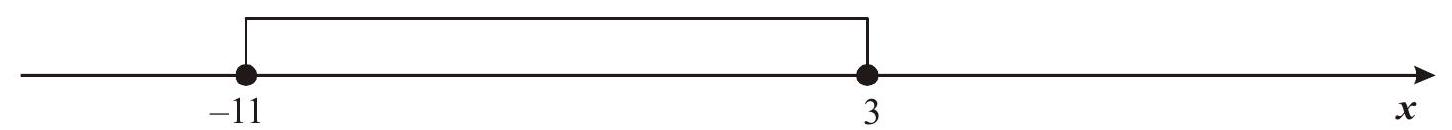
\includegraphics[max width=\textwidth, center]{2024_11_21_6a8be49478f78d0689cfg-02(1)}\\
B.\\
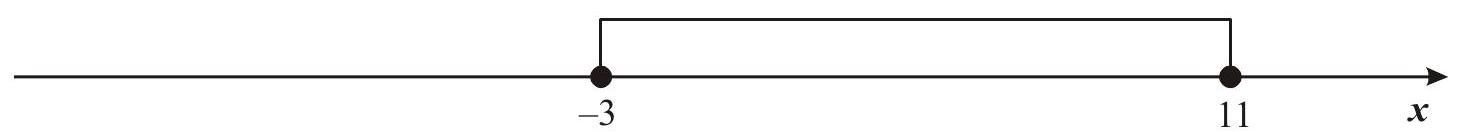
\includegraphics[max width=\textwidth, center]{2024_11_21_6a8be49478f78d0689cfg-02}\\
C.\\
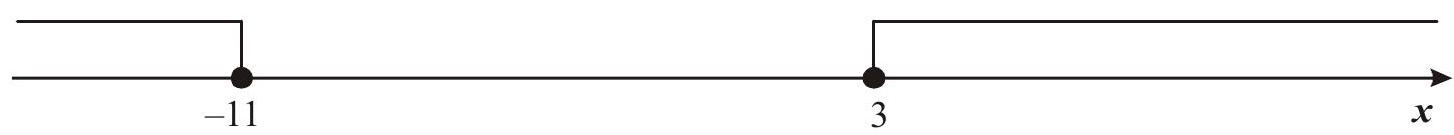
\includegraphics[max width=\textwidth, center]{2024_11_21_6a8be49478f78d0689cfg-02(2)}\\
D.\\
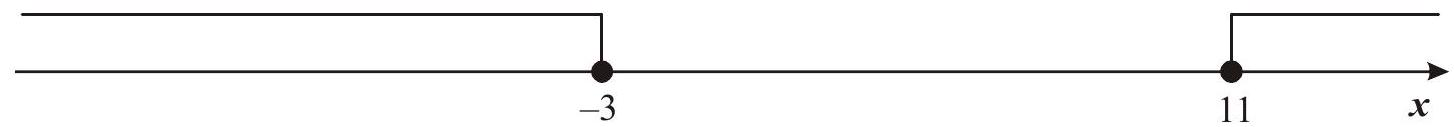
\includegraphics[max width=\textwidth, center]{2024_11_21_6a8be49478f78d0689cfg-02(3)}

\section*{BRUDNOPIS}
\begin{center}

\includegraphics[max width=\textwidth]{2024_11_21_6a8be49478f78d0689cfg-03}
\end{center}

\section*{Zadanie 7. (1 pkt)}
Dana jest parabola o równaniu \(y=x^{2}+8 x-14\). Pierwsza współzzędna wierzchołka tej paraboli jest równa\\
A. \(x=-8\)\\
B. \(x=-4\)\\
C. \(x=4\)\\
D. \(x=8\)

\section*{Zadanie 8. (1 pkt)}
Wskaż fragment wykresu funkcji kwadratowej, której zbiorem wartości jest \(\langle-2,+\infty)\).\\
A.\\
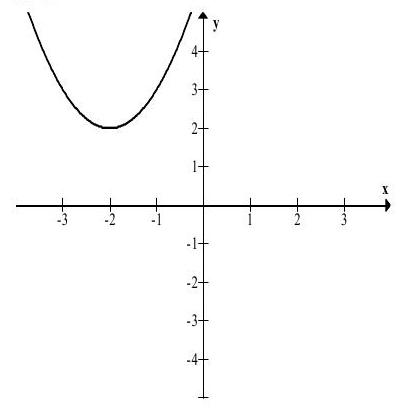
\includegraphics[max width=\textwidth, center]{2024_11_21_6a8be49478f78d0689cfg-04(2)}\\
B.\\
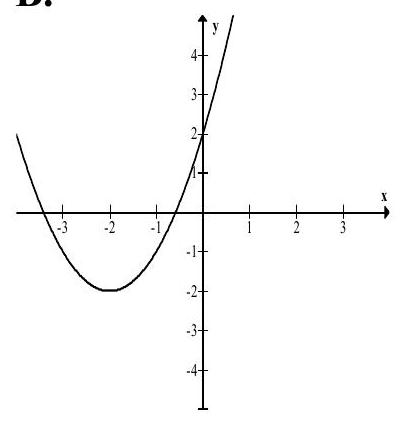
\includegraphics[max width=\textwidth, center]{2024_11_21_6a8be49478f78d0689cfg-04(1)}\\
C.\\
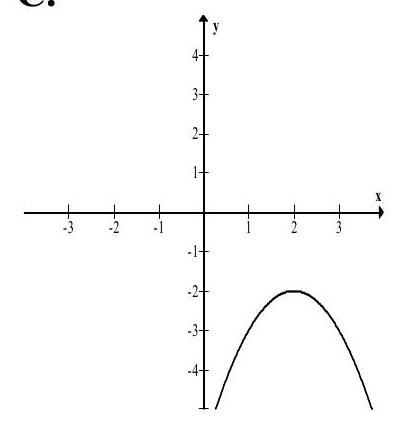
\includegraphics[max width=\textwidth, center]{2024_11_21_6a8be49478f78d0689cfg-04(3)}\\
D.\\
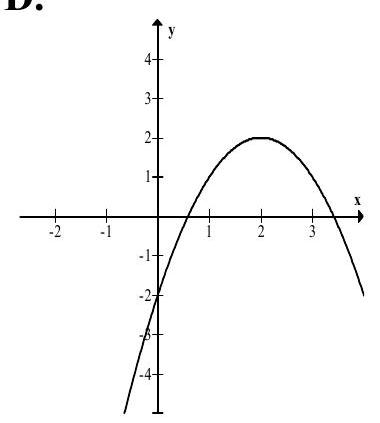
\includegraphics[max width=\textwidth, center]{2024_11_21_6a8be49478f78d0689cfg-04}

\section*{Zadanie 9. (1 pkt)}
Zbiorem rozwiązań nierówności \(x(x+6)<0\) jest\\
A. \((-6,0)\)\\
B. \((0,6)\)\\
C. \((-\infty,-6) \cup(0,+\infty)\)\\
D. \((-\infty, 0) \cup(6,+\infty)\)

\section*{Zadanie 10. (1 pkt)}
Wielomian \(W(x)=x^{6}+x^{3}-2\) jest równy iloczynowi\\
A. \(\left(x^{3}+1\right)\left(x^{2}-2\right)\)\\
B. \(\left(x^{3}-1\right)\left(x^{3}+2\right)\)\\
C. \(\left(x^{2}+2\right)\left(x^{4}-1\right)\)\\
D. \(\left(x^{4}-2\right)(x+1)\)

\section*{Zadanie 11. (1 pkt)}
Równanie \(\frac{(x+3)(x-2)}{(x-3)(x+2)}=0 \mathrm{ma}\)\\
A. dokładnie jedno rozwiazzanie\\
B. dokładnie dwa rozwiązania\\
C. dokładnie trzy rozwiazzania\\
D. dokładnie cztery rozwiązania

\section*{Zadanie 12. (1 pkt)}
Dany jest ciąg \(\left(a_{n}\right)\) określony wzorem \(a_{n}=\frac{n}{(-2)^{n}}\) dla \(n \geq 1\). Wówczas\\
A. \(a_{3}=\frac{1}{2}\)\\
B. \(a_{3}=-\frac{1}{2}\)\\
C. \(a_{3}=\frac{3}{8}\)\\
D. \(a_{3}=-\frac{3}{8}\)

\section*{BRUDNOPIS}
\begin{center}

\includegraphics[max width=\textwidth]{2024_11_21_6a8be49478f78d0689cfg-05}
\end{center}

\section*{Zadanie 13. (1 pkt)}
W ciagu geometrycznym \(\left(a_{n}\right)\) dane sa: \(a_{1}=36, a_{2}=18\). Wtedy\\
A. \(a_{4}=-18\)\\
B. \(a_{4}=0\)\\
C. \(a_{4}=4,5\)\\
D. \(a_{4}=144\)

\section*{Zadanie 14. (1 pkt)}
Kąt \(\alpha\) jest ostry i \(\sin \alpha=\frac{7}{13}\). Wtedy \(\operatorname{tg} \alpha\) jest równy\\
A. \(\frac{7}{6}\)\\
B. \(\frac{7 \cdot 13}{120}\)\\
C. \(\frac{7}{\sqrt{120}}\)\\
D. \(\frac{7}{13 \sqrt{120}}\)

\section*{Zadanie 15. (1 pkt)}
W trójkącie prostokątnym dane są długości boków (zobacz rysunek). Wtedy\\
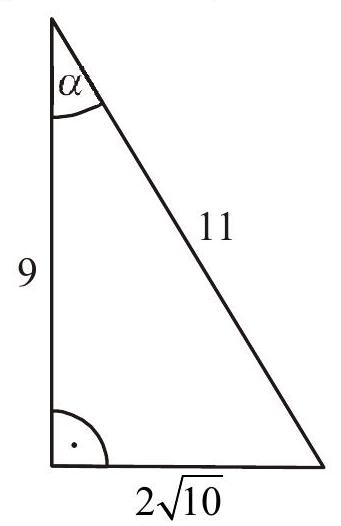
\includegraphics[max width=\textwidth, center]{2024_11_21_6a8be49478f78d0689cfg-06(1)}\\
A. \(\cos \alpha=\frac{9}{11}\)\\
B. \(\sin \alpha=\frac{9}{11}\)\\
C. \(\sin \alpha=\frac{11}{2 \sqrt{10}}\)\\
D. \(\cos \alpha=\frac{2 \sqrt{10}}{11}\)

\section*{Zadanie 16. (1 pkt)}
Przekątna \(A C\) prostokąta \(A B C D\) ma długość 14 . Bok \(A B\) tego prostokąta ma długość 6. Długość boku \(B C\) jest równa\\
A. 8\\
B. \(4 \sqrt{10}\)\\
C. \(2 \sqrt{58}\)\\
D. 10

\section*{Zadanie 17. (1 pkt)}
Punkty \(A, B\) i \(C\) leżą na okręgu o środku \(S\) (zobacz rysunek). Miara zaznaczonego kąta wpisanego \(A C B\) jest równa\\
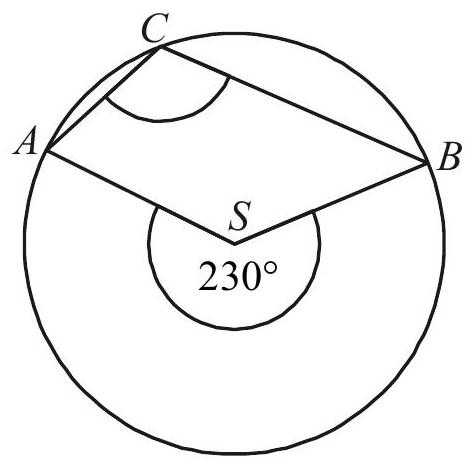
\includegraphics[max width=\textwidth, center]{2024_11_21_6a8be49478f78d0689cfg-06}\\
A. \(65^{\circ}\)\\
B. \(100^{\circ}\)\\
C. \(115^{\circ}\)\\
D. \(130^{\circ}\)

\section*{BRUDNOPIS}
\begin{center}

\includegraphics[max width=\textwidth]{2024_11_21_6a8be49478f78d0689cfg-07}
\end{center}

\section*{Zadanie 18. (1 pkt)}
Długość boku trójkąta równobocznego jest równa \(24 \sqrt{3}\). Promień okręgu wpisanego w ten trójkąt jest równy\\
A. 36\\
B. 18\\
C. 12\\
D. 6

\section*{Zadanie 19. (1 pkt)}
Wskaż równanie prostej przechodzącej przez początek układu współrzędnych i prostopadłej do prostej o równaniu \(y=-\frac{1}{3} x+2\).\\
A. \(y=3 x\)\\
B. \(y=-3 x\)\\
C. \(y=3 x+2\)\\
D. \(y=\frac{1}{3} x+2\)

\section*{Zadanie 20. (1 pkt)}
Punkty \(B=(-2,4)\) i \(C=(5,1)\) są dwoma sąsiednimi wierzchołkami kwadratu \(A B C D\). Pole tego kwadratu jest równe\\
A. 74\\
B. 58\\
C. 40\\
D. 29

\section*{Zadanie 21. (1 pkt)}
Dany jest okrąg o równaniu \((x+4)^{2}+(y-6)^{2}=100\). Środek tego okręgu ma współrzędne\\
A. \((-4,-6)\)\\
B. \((4,6)\)\\
C. \((4,-6)\)\\
D. \((-4,6)\)

\section*{Zadanie 22. (1 pkt)}
Objętość sześcianu jest równa 64. Pole powierzchni całkowitej tego sześcianu jest równe\\
A. 512\\
B. 384\\
C. 96\\
D. 16

\section*{Zadanie 23. (1 pkt)}
Przekrój osiowy stożka jest trójkątem równobocznym o boku \(a\). Objętość tego stożka wyraża się wzorem\\
A. \(\frac{\sqrt{3}}{6} \pi a^{3}\)\\
B. \(\frac{\sqrt{3}}{8} \pi a^{3}\)\\
C. \(\frac{\sqrt{3}}{12} \pi a^{3}\)\\
D. \(\frac{\sqrt{3}}{24} \pi a^{3}\)

\section*{Zadanie 24. (1 pkt)}
Pewna firma zatrudnia 6 osób. Dyrektor zarabia \(8000 \mathrm{zł}\), a pensje pozostałych pracowników są równe: \(2000 \mathrm{zł}, 2800 \mathrm{zl}, 3400 \mathrm{zl}, 3600 \mathrm{zl}, 4200 \mathrm{zł}\). Mediana zarobków tych 6 osób jest równa\\
A. 3400 zt\\
B. 3500 zf\\
C. \(6000 \mathrm{zł}\)\\
D. \(7000 \mathrm{zł}\)

\section*{Zadanie 25. (1 pkt)}
Ze zbioru \(\{1,2,3,4,5,6,7,8,9,10,11,12,13,14,15\}\) wybieramy losowo jedną liczbę. Niech p oznacza prawdopodobieństwo otrzymania liczby podzielnej przez 4. Wówczas\\
A. \(p<\frac{1}{5}\)\\
B. \(p=\frac{1}{5}\)\\
C. \(p=\frac{1}{4}\)\\
D. \(\quad p>\frac{1}{4}\)

\section*{BRUDNOPIS}
\begin{center}

\includegraphics[max width=\textwidth]{2024_11_21_6a8be49478f78d0689cfg-09}
\end{center}

\section*{ZADANIA OTWARTE}
\section*{Rozwiazania zadań o numerach od 26. do 34. należy zapisać w wyznaczonych miejscach pod treścia zadania.}
\section*{Zadanie 26. (2 pkt)}
Rozwiąż nierówność \(x^{2}-8 x+7 \geq 0\).

\begin{center}
\begin{tabular}{|c|c|c|c|c|c|c|c|c|c|c|c|c|c|c|c|c|c|c|c|c|c|c|c|c|c|c|c|c|c|c|}
\hline
 &  &  &  &  &  &  &  &  &  &  &  &  &  &  &  &  &  &  &  &  &  &  &  &  &  &  &  &  &  &  \\
\hline
 &  &  &  &  &  &  &  &  &  &  &  &  &  &  &  &  &  &  &  &  &  &  &  &  &  &  &  &  &  &  \\
\hline
 &  &  &  &  &  &  &  &  &  &  &  &  &  &  &  &  &  &  &  &  &  &  &  &  &  &  &  &  &  &  \\
\hline
 &  &  &  &  &  &  &  &  &  &  &  &  &  &  &  &  &  &  &  &  &  &  &  &  &  &  &  &  &  &  \\
\hline
 &  &  &  &  &  &  &  &  &  &  &  &  &  &  &  &  &  &  &  &  &  &  &  &  &  &  &  &  &  &  \\
\hline
 &  &  &  &  &  &  &  &  &  &  &  &  &  &  &  &  &  &  &  &  &  &  &  &  &  &  &  &  &  &  \\
\hline
 &  &  &  &  &  &  &  &  &  &  &  &  &  &  &  &  &  &  &  &  &  &  &  &  &  &  &  &  &  &  \\
\hline
 &  &  &  &  &  &  &  &  &  &  &  &  &  &  &  &  &  &  &  &  &  &  &  &  &  &  &  &  &  &  \\
\hline
 &  &  &  &  &  &  &  &  &  &  &  &  &  &  &  &  &  &  &  &  &  &  &  &  &  &  &  &  &  &  \\
\hline
 &  &  &  &  &  &  &  &  &  &  &  &  &  &  &  &  &  &  &  &  &  &  &  &  &  &  &  &  &  &  \\
\hline
 &  &  &  &  &  &  &  &  &  &  &  &  &  &  &  &  &  &  &  &  &  &  &  &  &  &  &  &  &  &  \\
\hline
 &  &  &  &  &  &  &  &  &  &  &  &  &  &  &  &  &  &  &  &  &  &  &  &  &  &  &  &  &  &  \\
\hline
 &  &  &  &  &  &  &  &  &  &  &  &  &  &  &  &  &  &  &  &  &  &  &  &  &  &  &  &  &  &  \\
\hline
 &  &  &  &  &  &  &  &  &  &  &  &  &  &  &  &  &  &  &  &  &  &  &  &  &  &  &  &  &  &  \\
\hline
 &  &  &  &  &  &  &  &  &  &  &  &  &  &  &  &  &  &  &  &  &  &  &  &  &  &  &  &  &  &  \\
\hline
 &  &  &  &  &  &  &  &  &  &  &  &  &  &  &  &  &  &  &  &  &  &  &  &  &  &  &  &  &  &  \\
\hline
 &  &  &  &  &  &  &  &  &  &  &  &  &  &  &  &  &  &  &  &  &  &  &  &  &  &  &  &  &  &  \\
\hline
\end{tabular}
\end{center}

Odpowiedź:\\
Zadanie 27. (2 pkt)\\
Rozwiąż równanie \(x^{3}-6 x^{2}-9 x+54=0\).\\

\includegraphics[max width=\textwidth, center]{2024_11_21_6a8be49478f78d0689cfg-10}

Odpowiedź:

\section*{Zadanie 28. (2 pkt)}
Pierwszy wyraz ciagu arytmetycznego jest równy 3, czwarty wyraz tego ciagu jest równy 15. Oblicz sumę sześciu początkowych wyrazów tego ciagu.\\

\includegraphics[max width=\textwidth, center]{2024_11_21_6a8be49478f78d0689cfg-11(1)}

Odpowiedź:

\section*{Zadanie 29. (2 pkt)}
W trójkącie równoramiennym \(A B C\) dane sa \(|A C|=|B C|=6\) i \(|\Varangle A C B|=30^{\circ}\) (zobacz rysunek). Oblicz wysokość \(A D\) trójkąta opuszczoną z wierzchołka \(A\) na bok \(B C\).\\
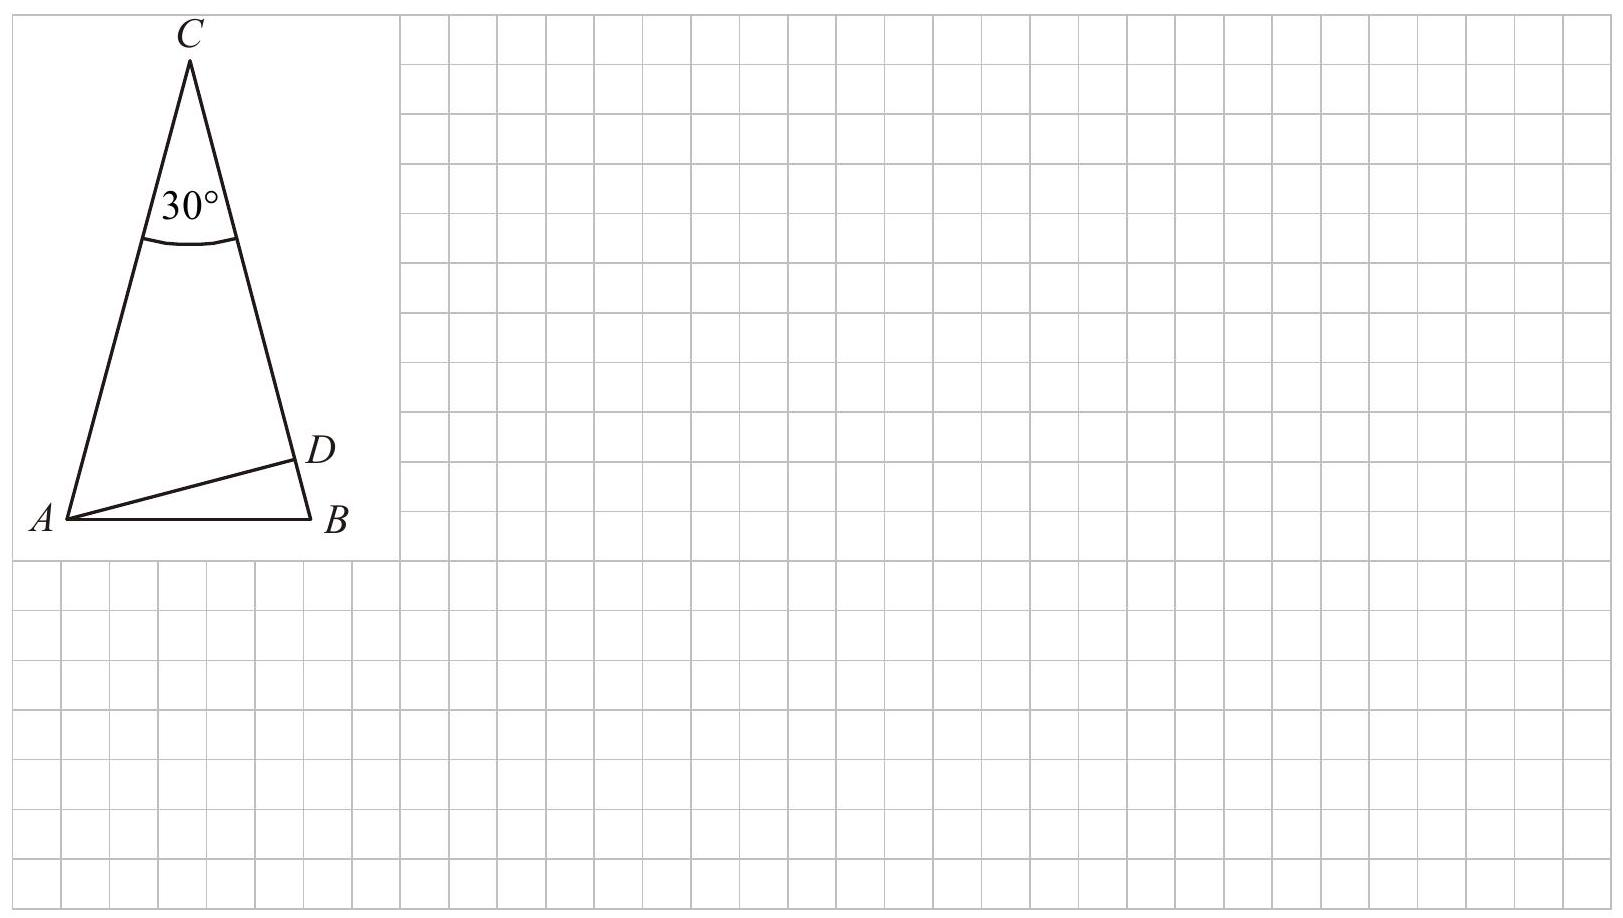
\includegraphics[max width=\textwidth, center]{2024_11_21_6a8be49478f78d0689cfg-11}

Odpowiedź:

\section*{Zadanie 30. (2 pkt)}
Dany jest równoległobok \(A B C D\). Na przedłużeniu przekątnej \(A C\) wybrano punkt \(E\) tak, że \(|C E|=\frac{1}{2}|A C|\) (zobacz rysunek). Uzasadnij, że pole równoległoboku \(A B C D\) jest cztery razy większe od pola trójkąta \(D C E\).\\

\includegraphics[max width=\textwidth, center]{2024_11_21_6a8be49478f78d0689cfg-12}

\section*{Zadanie 31. (2 pkt)}
Wykaż, że jeżeli \(c<0\), to trójmian kwadratowy \(y=x^{2}+b x+c\) ma dwa różne miejsca zerowe.

\begin{center}
\begin{tabular}{|c|c|c|c|c|c|c|c|c|c|c|c|c|c|c|c|c|c|c|c|c|c|c|}
\hline
 &  &  &  &  &  &  &  &  &  &  &  &  &  &  &  &  &  &  &  &  &  &  \\
\hline
 &  &  &  &  &  &  &  &  &  &  &  &  &  &  &  &  &  &  &  &  &  &  \\
\hline
 &  &  &  &  &  &  &  &  &  &  &  &  &  &  &  &  &  &  &  &  &  &  \\
\hline
 &  &  &  &  &  &  &  &  &  &  &  &  &  &  &  &  &  &  &  &  &  &  \\
\hline
 &  &  &  &  &  &  &  &  &  &  &  &  &  &  &  &  &  &  &  &  &  &  \\
\hline
 &  &  &  &  &  &  &  &  &  &  &  &  &  &  &  &  &  &  &  &  &  &  \\
\hline
 &  &  &  &  &  &  &  &  &  &  &  &  &  &  &  &  &  &  &  &  &  &  \\
\hline
 &  &  &  &  &  &  &  &  &  &  &  &  &  &  &  &  &  &  &  &  &  &  \\
\hline
 &  &  &  &  &  &  &  &  &  &  &  &  &  &  &  &  &  &  &  &  &  &  \\
\hline
 &  &  &  &  &  &  &  &  &  &  &  &  &  &  &  &  &  &  &  &  &  &  \\
\hline
 &  &  &  &  &  &  &  &  &  &  &  &  &  &  &  &  &  &  &  &  &  &  \\
\hline
 &  &  &  &  &  &  &  &  &  &  &  &  &  &  &  &  &  &  &  &  &  &  \\
\hline
 &  &  &  &  &  &  &  &  &  &  &  &  &  &  &  &  &  &  &  &  &  &  \\
\hline
 &  &  &  &  &  &  &  &  &  &  &  &  &  &  &  &  &  &  &  &  &  &  \\
\hline
 &  &  &  &  &  &  &  &  &  &  &  &  &  &  &  &  &  &  &  &  &  &  \\
\hline
 &  &  &  &  &  &  &  &  &  &  &  &  &  &  &  &  &  &  &  &  &  &  \\
\hline
 &  &  &  &  &  &  &  &  &  &  &  &  &  &  &  &  &  &  &  &  &  &  \\
\hline
 &  &  &  &  &  &  &  &  &  &  &  &  &  &  &  &  &  &  &  &  &  &  \\
\hline
 &  &  &  &  &  &  &  &  &  &  &  &  &  &  &  &  &  &  &  &  &  &  \\
\hline
 &  &  &  &  &  &  &  &  &  &  &  &  &  &  &  &  &  &  &  &  &  &  \\
\hline
 &  &  &  &  &  &  &  &  &  &  &  &  &  &  &  &  &  &  &  &  &  &  \\
\hline
 &  &  &  &  &  &  &  &  &  &  &  &  &  &  &  &  &  &  &  &  &  &  \\
\hline
 &  &  &  &  &  &  &  &  &  &  &  &  &  &  &  &  &  &  &  &  &  &  \\
\hline
 &  &  &  &  &  &  &  &  &  &  &  &  &  &  &  &  &  &  &  &  &  &  \\
\hline
 &  &  &  &  &  &  &  &  &  &  &  &  &  &  &  &  &  &  &  &  &  &  \\
\hline
 &  &  &  &  &  &  &  &  &  &  &  &  &  &  &  &  &  &  &  &  &  &  \\
\hline
 &  &  &  &  &  &  &  &  &  &  &  &  &  &  &  &  &  &  &  &  &  &  \\
\hline
 &  &  &  &  &  &  &  &  &  &  &  &  &  &  &  &  &  &  &  &  &  &  \\
\hline
 &  &  &  &  &  &  &  &  &  &  &  &  &  &  &  &  &  &  &  &  &  &  \\
\hline
 &  &  &  &  &  &  &  &  &  &  &  &  &  &  &  &  &  &  &  &  &  &  \\
\hline
 &  &  &  &  &  &  &  &  &  &  &  &  &  &  &  &  &  &  &  &  &  &  \\
\hline
 &  &  &  &  &  &  &  &  &  &  &  &  &  &  &  &  &  &  &  &  &  &  \\
\hline
 &  &  &  &  &  &  &  &  &  &  &  &  &  &  &  &  &  &  &  &  &  &  \\
\hline
 &  &  &  &  &  &  &  &  &  &  &  &  &  &  &  &  &  &  &  &  &  &  \\
\hline
 &  &  &  &  &  &  &  &  &  &  &  &  &  &  &  &  &  &  &  &  &  &  \\
\hline
 &  &  &  &  &  &  &  &  &  &  &  &  &  &  &  &  &  &  &  &  &  &  \\
\hline
 &  &  &  &  &  &  &  &  &  &  &  &  &  &  &  &  &  &  &  &  &  &  \\
\hline
 &  &  &  &  &  &  &  &  &  &  &  &  &  &  &  &  &  &  &  &  &  &  \\
\hline
 &  &  &  &  &  &  &  &  &  &  &  &  &  &  &  &  &  &  &  &  &  &  \\
\hline
 &  &  &  &  &  &  &  &  &  &  &  &  &  &  &  &  &  &  &  &  &  &  \\
\hline
 &  &  &  &  &  &  &  &  &  &  &  &  &  &  &  &  &  &  &  &  &  &  \\
\hline
 &  &  &  &  &  &  &  &  &  &  &  &  &  &  &  &  &  &  &  &  &  &  \\
\hline
 &  &  &  &  &  &  &  &  &  &  &  &  &  &  &  &  &  &  &  &  &  &  \\
\hline
 &  &  &  &  &  &  &  &  &  &  &  &  &  &  &  &  &  &  &  &  &  &  \\
\hline
\end{tabular}
\end{center}

\section*{Zadanie 32. (4 pkt)}
Dany jest trójkąt równoramienny \(A B C\), w którym \(|A C|=|B C|\) oraz \(A=(2,1)\) i \(C=(1,9)\).\\
Podstawa \(A B\) tego trójkąta jest zawarta w prostej \(y=\frac{1}{2} x\). Oblicz współrzędne wierzchołka \(B\).\\

\includegraphics[max width=\textwidth, center]{2024_11_21_6a8be49478f78d0689cfg-14}\\

\includegraphics[max width=\textwidth, center]{2024_11_21_6a8be49478f78d0689cfg-15}

Odpowiedź:

\section*{Zadanie 33. (4 pkt)}
W ostrosłupie prawidłowym czworokątnym \(A B C D S\) o podstawie \(A B C D\) i wierzchołku \(S\) trójkąt \(A C S\) jest równoboczny i ma bok długości 8 . Oblicz sinus kąta nachylenia ściany bocznej do płaszczyzny podstawy tego ostrosłupa (zobacz rysunek).\\
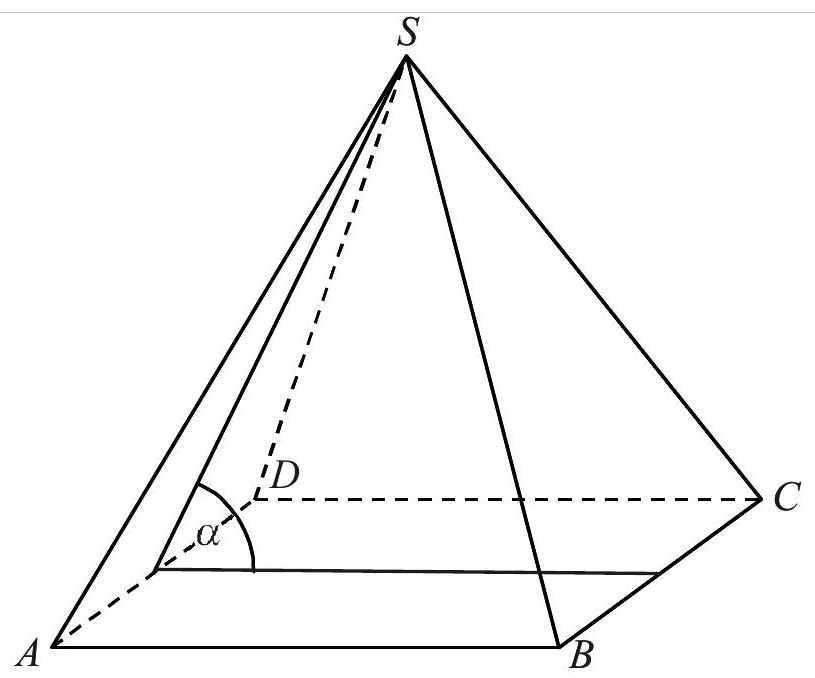
\includegraphics[max width=\textwidth, center]{2024_11_21_6a8be49478f78d0689cfg-16}\\

\includegraphics[max width=\textwidth, center]{2024_11_21_6a8be49478f78d0689cfg-16(1)}\\

\includegraphics[max width=\textwidth, center]{2024_11_21_6a8be49478f78d0689cfg-16(2)}\\

\includegraphics[max width=\textwidth, center]{2024_11_21_6a8be49478f78d0689cfg-17}

Odpowiedź:

\section*{Zadanie 34. (5 pkt)}
Kolarz pokonał trasę 114 km . Gdyby jechał ze średnią prędkością mniejszą o \(9,5 \mathrm{~km} / \mathrm{h}\), to pokonałby tę trasę w czasie o 2 godziny dłuższym. Oblicz, z jaką średnią prędkością jechał ten kolarz.

\begin{center}
\begin{tabular}{|c|c|c|c|c|c|c|c|c|c|c|c|c|c|c|c|c|c|c|c|c|c|c|}
\hline
 &  &  &  &  &  &  &  &  &  &  &  &  &  &  &  &  &  &  &  &  &  &  \\
\hline
 &  &  &  &  &  &  &  &  &  &  &  &  &  &  &  &  &  &  &  &  &  &  \\
\hline
 &  &  &  &  &  &  &  &  &  &  &  &  &  &  &  &  &  &  &  &  &  &  \\
\hline
 &  &  &  &  &  &  &  &  &  &  &  &  &  &  &  &  &  &  &  &  &  &  \\
\hline
 &  &  &  &  &  &  &  &  &  &  &  &  &  &  &  &  &  &  &  &  &  &  \\
\hline
 &  &  &  &  &  &  &  &  &  &  &  &  &  &  &  &  &  &  &  &  &  &  \\
\hline
 &  &  &  &  &  &  &  &  &  &  &  &  &  &  &  &  &  &  &  &  &  &  \\
\hline
 &  &  &  &  &  &  &  &  &  &  &  &  &  &  &  &  &  &  &  &  &  &  \\
\hline
 &  &  &  &  &  &  &  &  &  &  &  &  &  &  &  &  &  &  &  &  &  &  \\
\hline
 &  &  &  &  &  &  &  &  &  &  &  &  &  &  &  &  &  &  &  &  &  &  \\
\hline
 &  &  &  &  &  &  &  &  &  &  &  &  &  &  &  &  &  &  &  &  &  &  \\
\hline
 &  &  &  &  &  &  &  &  &  &  &  &  &  &  &  &  &  &  &  &  &  &  \\
\hline
 &  &  &  &  &  &  &  &  &  &  &  &  &  &  &  &  &  &  &  &  &  &  \\
\hline
 &  &  &  &  &  &  &  &  &  &  &  &  &  &  &  &  &  &  &  &  &  &  \\
\hline
 &  &  &  &  &  &  &  &  &  &  &  &  &  &  &  &  &  &  &  &  &  &  \\
\hline
 &  &  &  &  &  &  &  &  &  &  &  &  &  &  &  &  &  &  &  &  &  &  \\
\hline
 &  &  &  &  &  &  &  &  &  &  &  &  &  &  &  &  &  &  &  &  &  &  \\
\hline
 &  &  &  &  &  &  &  &  &  &  &  &  &  &  &  &  &  &  &  &  &  &  \\
\hline
 &  &  &  &  &  &  &  &  &  &  &  &  &  &  &  &  &  &  &  &  &  &  \\
\hline
 &  &  &  &  &  &  &  &  &  &  &  &  &  &  &  &  &  &  &  &  &  &  \\
\hline
 &  &  &  &  &  &  &  &  &  &  &  &  &  &  &  &  &  &  &  &  &  &  \\
\hline
 &  &  &  &  &  &  &  &  &  &  &  &  &  &  &  &  &  &  &  &  &  &  \\
\hline
 &  &  &  &  &  &  &  &  &  &  &  &  &  &  &  &  &  &  &  &  &  &  \\
\hline
 &  &  &  &  &  &  &  &  &  &  &  &  &  &  &  &  &  &  &  &  &  &  \\
\hline
 &  &  &  &  &  &  &  &  &  &  &  &  &  &  &  &  &  &  &  &  &  &  \\
\hline
 &  &  &  &  &  &  &  &  &  &  &  &  &  &  &  &  &  &  &  &  &  &  \\
\hline
 &  &  &  &  &  &  &  &  &  &  &  &  &  &  &  &  &  &  &  &  &  &  \\
\hline
 &  &  &  &  &  &  &  &  &  &  &  &  &  &  &  &  &  &  &  &  &  &  \\
\hline
 &  &  &  &  &  &  &  &  &  &  &  &  &  &  &  &  &  &  &  &  &  &  \\
\hline
 &  &  &  &  &  &  &  &  &  &  &  &  &  &  &  &  &  &  &  &  &  &  \\
\hline
 &  &  &  &  &  &  &  &  &  &  &  &  &  &  &  &  &  &  &  &  &  &  \\
\hline
 &  &  &  &  &  &  &  &  &  &  &  &  &  &  &  &  &  &  &  &  &  &  \\
\hline
 &  &  &  &  &  &  &  &  &  &  &  &  &  &  &  &  &  &  &  &  &  &  \\
\hline
 &  &  &  &  &  &  &  &  &  &  &  &  &  &  &  &  &  &  &  &  &  &  \\
\hline
 &  &  &  &  &  &  &  &  &  &  &  &  &  &  &  &  &  &  &  &  &  &  \\
\hline
 &  &  &  &  &  &  &  &  &  &  &  &  &  &  &  &  &  &  &  &  &  &  \\
\hline
 &  &  &  &  &  &  &  &  &  &  &  &  &  &  &  &  &  &  &  &  &  &  \\
\hline
 &  &  &  &  &  &  &  &  &  &  &  &  &  &  &  &  &  &  &  &  &  &  \\
\hline
 &  &  &  &  &  &  &  &  &  &  &  &  &  &  &  &  &  &  &  &  &  &  \\
\hline
 &  &  &  &  &  &  &  &  &  &  &  &  &  &  &  &  &  &  &  &  &  &  \\
\hline
 &  &  &  &  &  &  &  &  &  &  &  &  &  &  &  &  &  &  &  &  &  &  \\
\hline
 &  &  &  &  &  &  &  &  &  &  &  &  &  &  &  &  &  &  &  &  &  &  \\
\hline
 &  &  &  &  &  &  &  &  &  &  &  &  &  &  &  &  &  &  &  &  &  &  \\
\hline
 &  &  &  &  &  &  &  &  &  &  &  &  &  &  &  &  &  &  &  &  &  &  \\
\hline
\end{tabular}
\end{center}

\begin{center}

\includegraphics[max width=\textwidth]{2024_11_21_6a8be49478f78d0689cfg-19}
\end{center}

Odpowiedź:

\section*{BRUDNOPIS}

\end{document}